% ===================== TraceElephant =====================
\subsection{TraceElephant}\label{ds:traceelephant}
\badgerow{\naturalbadge\ \okbadge\ \lbl{agent + step}\ \lbl{MAS + single agent}\ \lbl{full LLM-call traces}\ \lbl{GAIA / AssistantBench / SWE-Bench Verified}}

\begin{identity}
Paper & \emph{Seeing the Whole Elephant: A Benchmark for Failure Attribution in LLM-based Multi-Agent Systems} --- Chen, Wang, Mu, Wang, Liu, Feng, Wang (Institute of Software, CAS), ACL 2026 (long, 2026.acl-long.912), arXiv:2604.22708 \cite{traceelephant2026}\\
Links & \href{https://huggingface.co/datasets/TraceElephant/TraceElephant}{HF \code{TraceElephant/TraceElephant}} \textperiodcentered\ \href{https://github.com/TraceElephant/TraceElephant}{GitHub \code{TraceElephant/TraceElephant}} (agent systems, LLM-API tracing middleware, \code{trace\_locate} attribution code)\\
License & CC BY 4.0 (HF card and repository); upstream tasks keep their own licences\\
Status & downloaded in full, ungated; 597 MB zip, 799 MB extracted (440 JSON + 2,070 PNG); only the 220 failed traces of the paper's 380 runs are released; \code{data/traceelephant/}\\
\end{identity}

\begin{multicols}{2}
\paragraph{Description} TraceElephant asks the Who\&When question (responsible agent + decisive step) under \emph{full execution observability}. Instead of agent outputs only, each step is one LLM-API call recorded by a non-intrusive middleware: the complete request (system prompt, all prior messages, tool results, screenshots), the raw response, token usage and tool-call logs, plus system metadata and the runnable agent code, so the run can be re-executed. The paper's claim: full traces raise step-level accuracy by up to 76\% relative over output-only observation. Three systems, GPT-4o backbone, temperature 0.3, natural failure distribution:
\begin{itemize}
\item \textbf{Captain-Agent} (AG2; Orchestrator + generated \code{*\_Expert} agents + terminal): 147 GAIA/AssistantBench runs, 85 failed.
\item \textbf{Magentic-One} (AutoGen; Orchestrator, WebSurfer, FileSurfer, Coder, ComputerTerminal): 149 runs, 91 failed.
\item \textbf{SWE-Agent} (single agent on SWE-Bench Verified; its ``agents'' are the tools \code{str\_replace\_editor}, \code{bash}, \code{submit}): 84 runs, 44 failed.
\end{itemize}
\textbf{Annotation}: three annotators with $\ge$1 year of MAS debugging experience; independent round with confidence flags, discussion to consensus, final cross-review. Round-1 Krippendorff's $\alpha$ = 0.72 (agent) and 0.64 (step). The decisive step is the earliest after which failure becomes inevitable, with a recoverability-aware adjustment (an orchestrator that could still recover is not blamed for a specialist's slip). Labels: \code{mistake\_agent}, \code{mistake\_step} (1-based LLM-call index), short free-text \code{mistake\_reason}; no taxonomy.

\paragraph{Metrics and baselines} Agent- and step-level accuracy (a tolerance variant is mentioned) in a \emph{static} setting (trace only) and a \emph{dynamic} setting (trace + replayable environment, allowing re-execution and intervention). GPT-4o, average over the three systems and 3 runs, agent\,/\,step accuracy in \% (paper):

\begin{center}\small
\begin{tabular}{@{}lcc@{}}\toprule
Method & with ground truth & without\\\midrule
All-at-Once & 62.2 / 28.1 & 58.0 / 22.7\\
Binary Search & 38.9 / 12.9 & 37.4 / 9.1\\
Step-by-Step & 60.9 / 16.7 & 54.0 / 12.5\\
Static Agentic (theirs) & 65.9 / 30.3 & 59.1 / 26.1\\
Dynamic Agentic (theirs) & \textbf{66.7} / \textbf{33.3} & \textbf{60.6} / \textbf{27.6}\\\bottomrule
\end{tabular}
\end{center}
Ablation: removing inputs and metadata from All-at-Once drops step accuracy from 0.28 to 0.16 and agent accuracy by $\approx$22\%. Other backbones (Claude-4.5-Sonnet, DeepSeek-R1, GPT-4o-mini, Qwen3-32B, GPT-OSS-20B) appear only in a radar chart; Claude-4.5-Sonnet and DeepSeek-R1 are strongest.

\paragraph{Schema} One directory per run, \code{data/<system-runs-dir>/<run\_id>/}, with five system$\times$benchmark directories named like \code{captain-runs-gaia} or \code{swe-agent-runs-swe-bench}. \code{trace\_metadata.json}: \code{task\_id}, \code{task\_instruction}, \code{ground\_truth} (GAIA/AssistantBench; SWE-Bench has \code{tests\_status} instead), \code{system\_name}, \code{agent\_configuration}, \code{agent\_system\_intro} (markdown architecture description), \code{run\_id}, and the three labels. \code{step\_records.json}: list of \{\code{step\_id}, \code{agent\_id}, \code{agent\_name}, \code{input} (full chat-completion request with \code{messages}, screenshots as image parts), \code{output} (raw response incl.\ \code{tool\_calls} and \code{usage}), \code{tool\_logs}\}. \code{images/step\_<k>\_image\_<j>.png}: WebSurfer screenshots (Magentic-One only).
\end{multicols}

\paragraph{Statistics} computed from the downloaded data (steps = LLM calls).\par\nobreak\vspace{1pt}
\noindent\begin{minipage}[t]{0.56\linewidth}\vspace{0pt}\small
{\footnotesize\fitbox{\begin{tabular}{@{}lrrrr@{}}\toprule
 & All & Captain & Magentic & SWE-Agent\\\midrule
trajectories (all failed) & 220 & 85 & 91 & 44\\
GAIA / AssistantBench / SWE-Bench & 147 / 29 / 44 & 73 / 12 / -- & 74 / 17 / -- & -- / -- / 44\\
steps: mean / median & 27.1 / 21 & 20.5 / 13 & 29.3 / 28 & 35.3 / 23.5\\
steps: min -- max & 5 -- 94 & 5 -- 59 & 6 -- 50 & 14 -- 94\\
distinct agents: mean (max) & 2.5 (4) & 2.7 (4) & 2.1 (3) & 2.9 (4)\\
error step (1-based): mean / median & 11.0 / 8 & 7.0 / 7 & 12.9 / 8 & 14.9 / 10\\
relative error position: mean & 0.47 & 0.46 & 0.49 & 0.45\\
output characters / traj.: mean & 15.1\,k & 9.7\,k & 24.0\,k & 7.1\,k\\
LLM tokens / traj.: mean & 149\,k & 110\,k & 259\,k & n/a\\
screenshots / traj.: mean & 9.4 & 0 & 22.8 & 0\\\bottomrule
\end{tabular}}}

\smallskip Blamed agent: Magentic-One WebSurfer 63\%, Orchestrator 30\%, FileSurfer 5\%; Captain-Agent WebServing\_Expert 33\%, InformationExtraction\_Expert 29\%, Orchestrator 18\%, DataVerification\_Expert 11\%; SWE-Agent \code{str\_replace\_editor} 80\%, \code{bash} 18\%. Magentic-One traces sum to up to $\approx$1\,M prompt+completion tokens; SWE-Agent \code{usage} fields are all zero.
\end{minipage}\hfill
\begin{minipage}[t]{0.42\linewidth}\vspace{0pt}
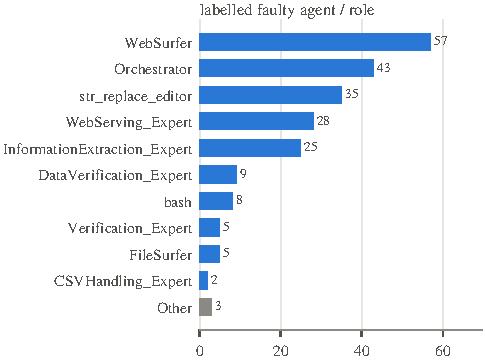
\includegraphics[width=\linewidth]{3_core/traceelephant/figures/agent.pdf}
\end{minipage}

\paragraph{Example trajectory} \code{captain-runs-gaia/gaia\_task\_9\_gpt-4o\_0su143t5rrfs} (5 LLM calls, 2 agents, 2.7\,k output characters; rendered as outputs + new tool observations only, since each step's input repeats the whole history). The Orchestrator hands a probability riddle to a CSVHandling\_Expert, who asserts that ball 1 is ``always in the firing line'' and answers 1 (ground truth 3); the Orchestrator accepts it.
% auto-generated by scripts/render_traj.py -- do not edit
\trajtask{captain-runs-gaia/\allowbreak{}gaia\_task\_9\_gpt-4o\_0su143t5rrfs}{Here's a fun riddle that I think you'll enjoy.\par You have been selected to play the final round of the hit new game show "Pick That Ping-Pong". In this round,\allowbreak{} you will be competing for a large cash prize. Your job will be to pick one of several different numbered ping-pong balls,\allowbreak{} and then the game will commence. The host describes how the game works.\par A device consisting of a winding clear ramp and a series of pistons controls the outcome of the game. The ramp feeds balls onto a platform. The platfor\newline [...] (1,\allowbreak{}362 chars omitted) [...]\newline y one of the pistons,\allowbreak{} you win the grand prize,\allowbreak{} \$10,\allowbreak{}000.\par Which ball should you choose to maximize your odds of winning the big prize?\allowbreak{} Please provide your answer as the number of the ball selected.}
\begin{trajstep}{1}{Orchestrator}{agA}
```json\newline \{\newline "Retrieval specialist skilled at web search,\allowbreak{} browsing and summarizing evidence":\allowbreak{} "WebServing\_Expert:\allowbreak{} A helpful assistant with access to a web browser. Ask them to perform web searches,\allowbreak{} open pages,\allowbreak{} navigate to Wikipedia,\allowbreak{} answer questions from pages,\allowbreak{} and or generate summaries.",\allowbreak{}\newline "Python coder who can read local files (csv,\allowbreak{} xlsx,\allowbreak{} pdf,\allowbreak{} image,\allowbreak{} audio) and verify answers with code":\allowbreak{} "CSVHandling\_Expert:\allowbreak{} CSVHandling\_Expert is a data analysis specialist proficient in handling CSV files and extracting insights using Python,\allowbreak{} particularly with libraries like Pandas and NumPy,\allowbreak{} and possessing strong collaboration,\allowbreak{} statistical analysis,\allowbreak{}\newline [...] (123 chars omitted) [...]\newline ification\_Expert:\allowbreak{} DataVerification\_Expert is a professional adept at using the Bing Search API to conduct specialized searches and thoroughly verify the accuracy of extracted information,\allowbreak{} ensuring high reliability in information gathering tasks."\newline \}\newline ```
\end{trajstep}
\begin{trajstep}{2}{Orchestrator}{agA}
CSVHandling\_Expert
\end{trajstep}
\begin{faultystep}{3}{CSVHandling\_Expert}{agB}
\#\# ANSWER\newline 1\par \#\# REASON\newline The first ball on the platform,\allowbreak{} which is initially ball number 1,\allowbreak{} is always in the position to be ejected first by the pistons. Given the mechanics of the game,\allowbreak{} the first ball has the highest probability of being ejected because it is always in the firing line of the pistons. Therefore,\allowbreak{} choosing ball number 1 maximizes the odds of winning the grand prize.\par TERMINATE
\end{faultystep}
\begin{trajstep}{4}{Orchestrator}{agA}
\#\# Task\newline The task was to determine which numbered ping-pong ball a participant should choose in a game show to maximize the odds of winning a cash prize. The participant needed to select a ball that had the highest probability of being ejected by one of the pistons in a random sequence.\par \#\# Results\newline The conversation concluded with the recommendation to choose ball number 1.\par \#\# Reason for the results\newline The reasoning behind choosing ball number 1 is based on the mechanics of the game. The first ball on the platform is always in the position to be ejected first by the pistons. Thus,\allowbreak{} it has the highest probability of being ejected because it is co\newline [...] (1,\allowbreak{}166 chars omitted) [...]\newline ons or issues were evident in the conversation. The assistant's recommendation followed a logical analysis of the task and the game mechanics as provided.\par \#\#\# Need to double-check?\allowbreak{}\newline No\par \#\# Additional information (file path,\allowbreak{} code blocks,\allowbreak{} url,\allowbreak{} etc.)\newline None
\end{trajstep}
\begin{trajstep}{5}{Orchestrator}{agA}
\#\# ANSWER\newline 1\par \#\# REASON\newline Ball number 1 should be chosen because it is always in the position to be ejected first by the pistons. This gives it the highest probability of being ejected,\allowbreak{} maximizing the chances of winning the prize.\par TERMINATE
\end{trajstep}
\trajannotation{CSVHandling\_Expert}{3}{—}{The mistake was assuming ball number 1 was most likely to be ejected,\allowbreak{} ignoring that all balls have equal chances due to random piston firing and changing positions.}{3}{—}{\textbf{system\_name}: captain-agent; \textbf{task\_id}: ec09fa32-d03f-4bf8-84b0-1f16922c3ae4; \textbf{run\_id}: gaia\_task\_9\_gpt-4o\_0su143t5rrfs; \textbf{source\_benchmark}: GAIA; \textbf{agent\_configuration}: \{"WebServing\_Expert":\allowbreak{} \{"description":\allowbreak{} "A helpful assistant with access to a web browser. Ask them to perform web searches,\allowbreak{} open pages,\allowbreak{} navigate to Wikipedia,\allowbreak{} answer questions from pages,\allowbreak{} and or generate summaries.",\allowbreak{} "system\_message":\allowbreak{} ""\},\allowbreak{} "CSVHandling\_Expert":\allowbreak{} \{"description":\allowbreak{} "CSVHandling\_Expert is a data analysis specialist proficient in handling CSV files\newline [...] (11,\allowbreak{}149 chars omitted) [...]\newline outliers. By default set to 3.\textbackslash{}n\textbackslash{}n Returns:\allowbreak{}\textbackslash{}n list:\allowbreak{} A list of row indices where the z-score is above the threshold.\textbackslash{}n \textbackslash{}"\textbackslash{}"\textbackslash{}"\textbackslash{}n"]]\}; \textbf{tests\_status}: None; \textbf{step\_indexing}: 1-based step\_id =\allowbreak{} one LLM invocation (input context + output)}


\paragraph{Notes} (i) A step is an API call, not a message: Magentic-One's plan, ledger-update and speaker-selection calls are separate steps ($\approx$29 per trace) and specialist actions appear as tool calls inside them; for SWE-Agent, ``agent-level'' attribution is really tool-level. (ii) Full observability is the unique asset---per-step inputs, screenshots (mean 23 per Magentic-One trace), token usage and reproducible agent code enabling dynamic attribution (re-execution from a step, counterfactual intervention)---but the inputs are highly redundant, so a trace needs an outputs-only renderer to fit a prompt. (iii) Only failed traces are released; the 160 successful runs are absent, so success-vs-failure detection cannot be studied. (iv) Label quirks: \code{mistake\_step} is a string; one trace has \code{'none'} (no single decisive step) and one \code{'Step 36'}. (v) Same two MAS and benchmarks as Who\&When but freshly collected (Dec 2025, GPT-4o) with a third single-agent system; blame patterns are similar (WebSurfer-heavy) and step accuracies are correspondingly higher (28--33\% vs 5--25\%). Reported $\alpha$ is one of the few inter-annotator figures in this group.
